As previously mentioned, the computational mesh velocity assumes 
different values of velocity from the Eulerian and Lagrangean 
description. Thus, it can be represented as a linear 
combination of other velocities, such as:

\begin{equation}
\hat{\textbf{v}} 
= \beta_{1} \textbf{v}_{1}
+ \beta_{2} \textbf{v}_{2}
\end{equation}

\medskip
\noindent
where,
$\textbf{v}_{1}$ is the Lagrangian velocity,
$\textbf{v}_{2}$ is the Laplacian smoothing velocity,
$\beta_{1}$ is a parameter controls the Lagragian motion and
$\beta_{2}$ controls the intensity of velocity smoothing.
The choice of these velocity fields and their parameters must 
be in order to improve the result of the numerical 
simulation and to avoid the degradation of the 
computational elements, especially close to the domain boundary, 
where the elements are compressed making the simulation unstable.

\medskip
Lagrangian velocity is the material flow velocity. 
This portion makes the nodes of the computational 
mesh move in the same direction and sense as the flow velocity. 
The intensity is proportional to the value of parameter $\beta_{1}$.
Depending on the chosen value, the insertion and deletion 
of nodes are required.

\medskip
The velocity of Laplacian smoothing is that nodes 
acquire due to their topological redistribution. 
Considering a node in a non-uniform mesh, it will be 
moved to the centroid of the 1-ring neighbors. 
Thereby, it is expected the smoothing procedure
converges to a more uniform point distribution,
as shown in \ref{laplacian smoothing space}.

\vspace{0.5cm}
\begin{figure}[H]
\begin{center}
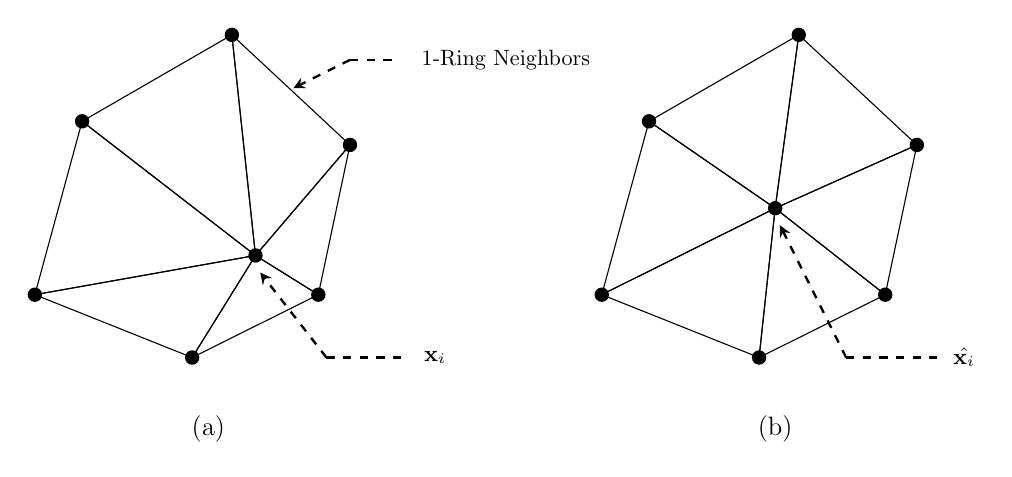
\begin{tikzpicture}[scale=6]

 % FIGURE A
 % nodes
 \coordinate (E) at (1.233,0.6830) {};
 \coordinate (F) at (1.333,1.0500) {};
 \coordinate (I) at (1.566,0.5500) {};
 \coordinate (J) at (1.7,0.7660) {};
 \coordinate (K) at (1.650,1.2330) {};
 \coordinate (N) at (1.833,0.6830) {};
 \coordinate (O) at (1.900,1.0000) {};



 % elements
 \draw (E) -- (J) -- (F) -- cycle;
 \draw (J) -- (K) -- (F) -- cycle;
 \draw (I) -- (N) -- (J) -- cycle;
 \draw (N) -- (O) -- (J) -- cycle;
 \draw (J) -- (O) -- (K) -- cycle;
 \draw (I) -- (J) -- (E) -- cycle;
 

 % draw nodes
 \node[circle, fill=black, inner sep=0pt, minimum size=5.2pt] at (E) {};
 \node[circle, fill=black, inner sep=0pt, minimum size=5.2pt] at (F) {};
 \node[circle, fill=black, inner sep=0pt, minimum size=5.2pt] at (I) {};
 \node[circle, fill=black, inner sep=0pt, minimum size=5.2pt] at (J) {};
 \node[circle, fill=black, inner sep=0pt, minimum size=5.2pt] at (K) {};
 \node[circle, fill=black, inner sep=0pt, minimum size=5.2pt] at (N) {};
 \node[circle, fill=black, inner sep=0pt, minimum size=5.2pt] at (O) {};



 % -----------------------------------------------------------------
 % FIGURE B
 % nodes
 \coordinate (E) at (2.433,0.6830) {};
 \coordinate (F) at (2.533,1.0500) {};
 \coordinate (I) at (2.766,0.5500) {};
 \coordinate (J) at (2.8,0.8660) {};
 \coordinate (K) at (2.850,1.2330) {};
 \coordinate (N) at (3.033,0.6830) {};
 \coordinate (O) at (3.100,1.0000) {};

 % elements
 \draw (E) -- (J) -- (F) -- cycle;
 \draw (J) -- (K) -- (F) -- cycle;
 \draw (I) -- (N) -- (J) -- cycle;
 \draw (N) -- (O) -- (J) -- cycle;
 \draw (J) -- (O) -- (K) -- cycle;
 \draw (I) -- (J) -- (E) -- cycle;
 

 % draw nodes
 \node[circle, fill=black, inner sep=0pt, minimum size=5.2pt] at (E) {};
 \node[circle, fill=black, inner sep=0pt, minimum size=5.2pt] at (F) {};
 \node[circle, fill=black, inner sep=0pt, minimum size=5.2pt] at (I) {};
 \node[circle, fill=black, inner sep=0pt, minimum size=5.2pt] at (J) {};
 \node[circle, fill=black, inner sep=0pt, minimum size=5.2pt] at (K) {};
 \node[circle, fill=black, inner sep=0pt, minimum size=5.2pt] at (N) {};
 \node[circle, fill=black, inner sep=0pt, minimum size=5.2pt] at (O) {};


 % arrow and legend
 \draw[dashed,line width=0.03cm,-stealth] (1.85,0.55) -- (1.71,0.73);
 \draw[dashed,line width=0.03cm] (1.85,0.55) -- (2.015,0.55);
 \node[draw=none, scale=0.9] at (2.08,0.55) {\small $\textbf{x}_{i}$};
 
 \draw[dashed,line width=0.03cm,-stealth] (2.95,0.55) -- (2.81,0.83);
 \draw[dashed,line width=0.03cm] (2.95,0.55) -- (3.15,0.55);
 \node[draw=none, scale=0.9] at (3.2,0.55) {\small $\hat{\textbf{x}_{i}}$};
 
 \draw[dashed,line width=0.03cm,-stealth] (1.9,1.18) -- (1.78,1.12);
 \draw[dashed,line width=0.03cm] (1.9,1.18) -- (2.0,1.18);
 \node[draw=none,align=center,scale=0.8] at (2.23,1.18) {1-Ring Neighbors};

 \node[draw=none, scale=0.8] at (1.6,0.4) {\large (a)};
 \node[draw=none, scale=0.8] at (2.8,0.4) {\large (b)};


 
\end{tikzpicture}
\end{center}
\caption{Laplacian smoothing in 2-dimensional space: 
(a) initial point position and
(b) final point position after successively smoothing steps.
}
\label{laplacian smoothing space}
\end{figure}




\medskip
According to \cite{zheng1996}, the new node position 
$\hat{\textbf{x}}_{i}$ can be approximated using an 
iterative weighted sum
of the 1-ring neighbors of a node:

\begin{equation}
\hat{\textbf{x}}_{i} 
= \sum_{i}^{np} \sum_{j}^{N_1} w_{ij}
\left( \textbf{x}_{j} - \textbf{x}_{i} \right)
\end{equation}

\medskip
\noindent
where, 
$w_{ij}$ is the weight and it can be calculated in several ways,
$np$ is number of computational mesh node,
$N_{1}$ is the 1-ring neighbors of a node,
$\textbf{x}_{j}$ is the coordinate vector of neighbor node and
$\textbf{x}_{i}$ is the coordinate vector of node in previous step that will be moved.
It is possible to choose several strategies to calculate 
the weight of this equation. In this work, the weight was 
calculated as the sum of the inverse distance from its neighbor vertices,
that is:
\begin{equation}
w_{ij} = \sum_{i}^{np} \sum_{j}^{N_1}
\frac{1}{\left( \textbf{x}_{j} - \textbf{x}_{i} \right)}
\end{equation}

\medskip
\noindent
Then, the Laplacian smoothing velocity can be calculated as:


\begin{equation}
\textbf{v}_{2}
= \sum_{i}^{np} \sum_{j}^{N_1} w_{ij}
\frac{\left( \textbf{x}_{j} - \textbf{x}_{i} \right)}{\Delta t}
\end{equation}

\medskip
In \ref{laplacian smoothing fig} is shown 
the Laplacian smoothing application in a moving boundary problem
when it tends to the maximum compression state.
As can be seen, the elements close to the boundary are compressed 
until they leave the domain (\ref{laplacian smoothing fig}a). 
However, this effect is not seen when 
Laplacian smoothing is applied (\ref{laplacian smoothing fig}b). 
In these cases, Laplacian smoothing becomes essential 
to perform the numerical simulation.


\begin{figure}[H]
     \begin{minipage}{.50\linewidth}
      \centering
      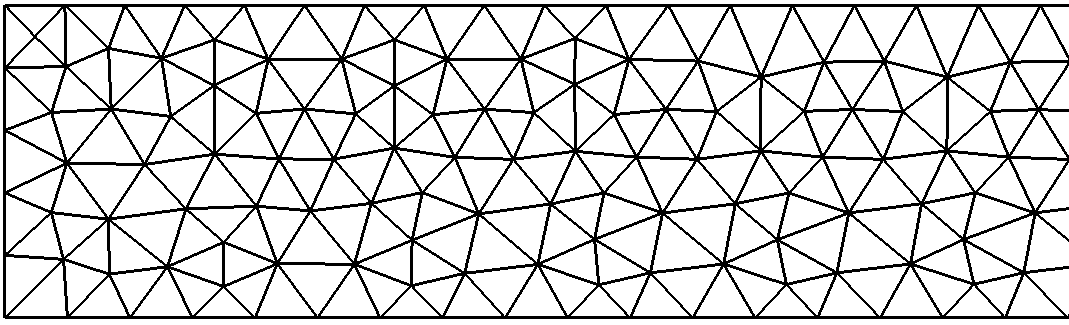
\includegraphics[scale=0.19]{./02_chaps/cap_numerico/figure/no1.png}\\
     \end{minipage}%
     \begin{minipage}{.50\linewidth}
      \centering
      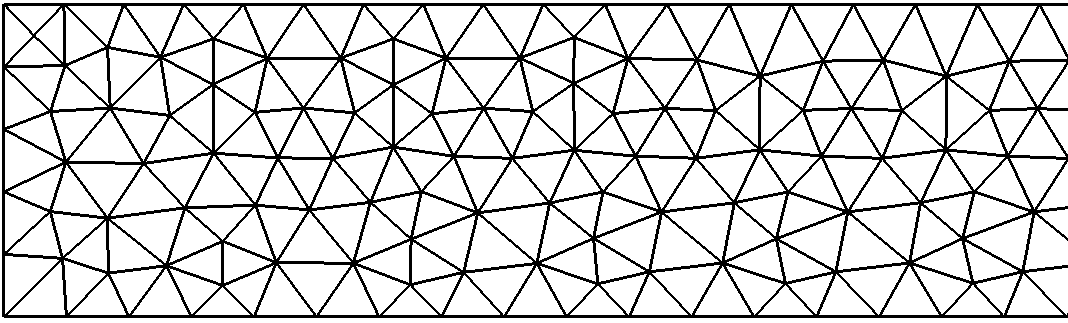
\includegraphics[scale=0.19]{./02_chaps/cap_numerico/figure/with1.png}\\
     \end{minipage}
     \begin{minipage}{.50\linewidth}
     \medskip
      \centering
      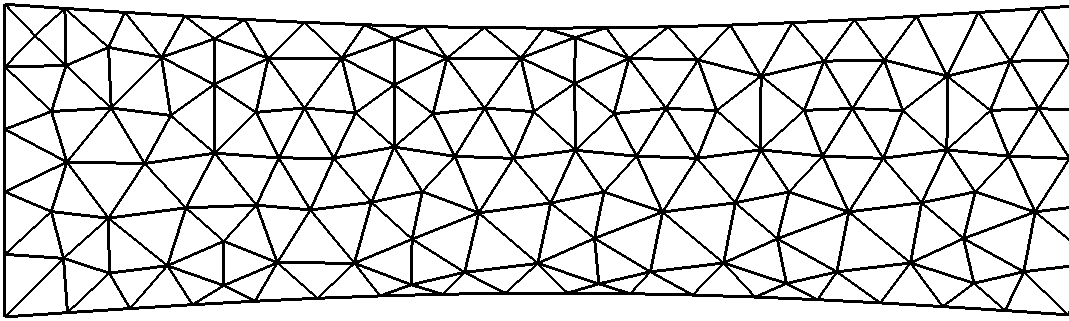
\includegraphics[scale=0.19]{./02_chaps/cap_numerico/figure/no2.png}\\
     \end{minipage}%
     \begin{minipage}{.50\linewidth}
     \medskip
      \centering
      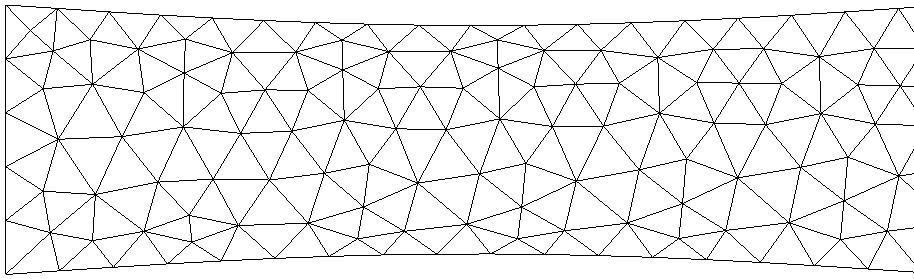
\includegraphics[scale=0.19]{./02_chaps/cap_numerico/figure/with2.png}\\
     \end{minipage}\\[7pt]
     \begin{minipage}{.50\linewidth}
      \centering
      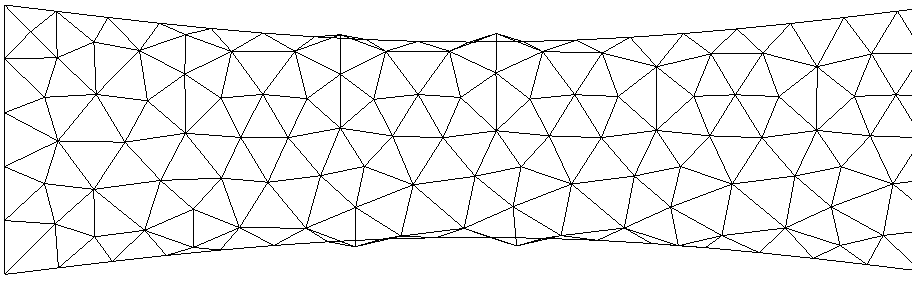
\includegraphics[scale=0.19]{./02_chaps/cap_numerico/figure/no3.png}\\
     \end{minipage}%
     \begin{minipage}{.50\linewidth}
      \centering
      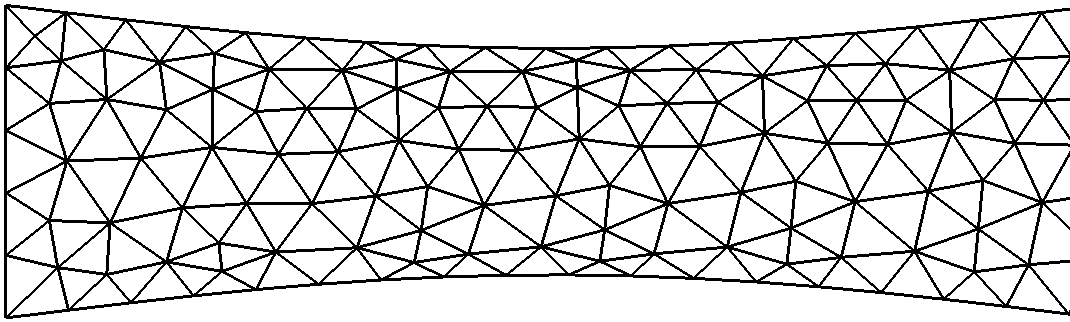
\includegraphics[scale=0.19]{./02_chaps/cap_numerico/figure/with3.png}\\
     \end{minipage}
     \begin{minipage}{.50\linewidth}
     \medskip
      \centering
      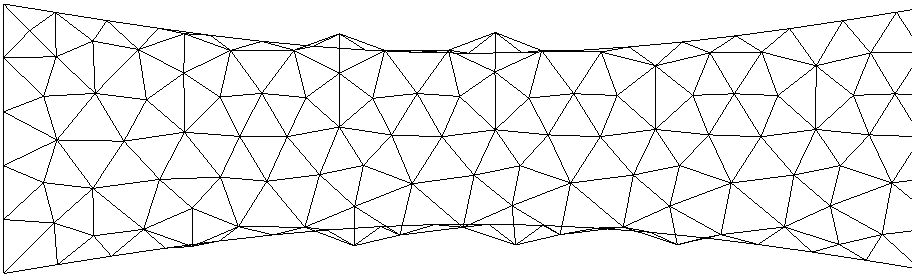
\includegraphics[scale=0.19]{./02_chaps/cap_numerico/figure/no4.png}\\
     \end{minipage}%
     \begin{minipage}{.50\linewidth}
     \medskip
      \centering
      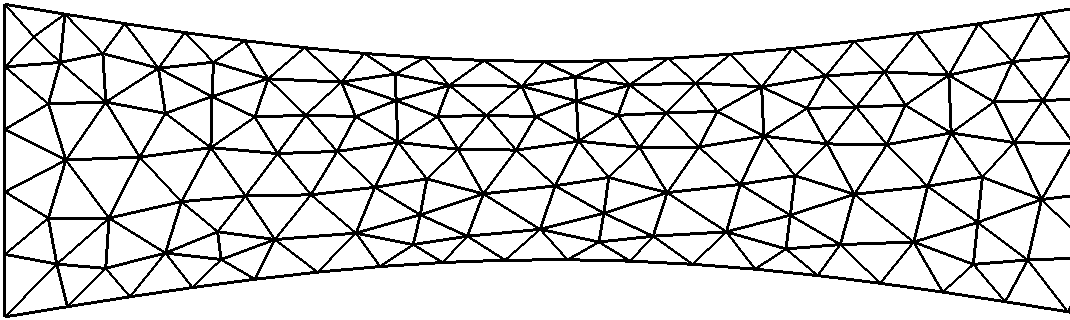
\includegraphics[scale=0.19]{./02_chaps/cap_numerico/figure/with4.png}\\
     \end{minipage}
     \medskip
     \caption{
The comparison for the same time step between 
     (a) no Laplacian smoothing and
     (b) with Laplacian smoothing
in a moving boundary problem.
}
     \label{laplacian smoothing fig}
\end{figure}



